% !TEX root = ../document.tex
% !TeX spellcheck = pt_BR

\section{Pré-processamento}

\begin{frame}{Pré-processamento -- Detecção QRS}
    \center
    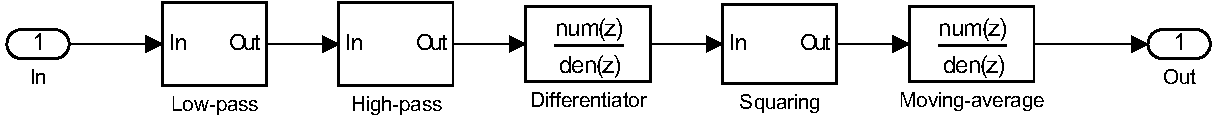
\includegraphics[scale=0.55]{figures/qrs-filter.pdf}
    \vskip10pt
    \begin{columns}[b]
        \hskip-15pt
        \column{0.1\textwidth}
        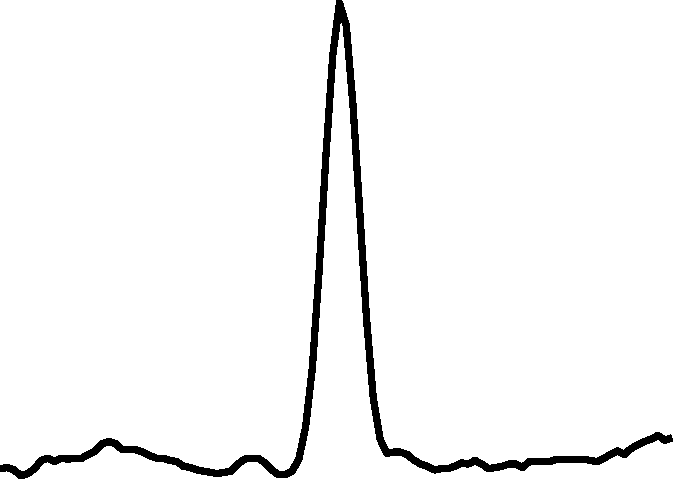
\includegraphics[scale=0.15]{figures/original.pdf}
        \column{0.1\textwidth}
        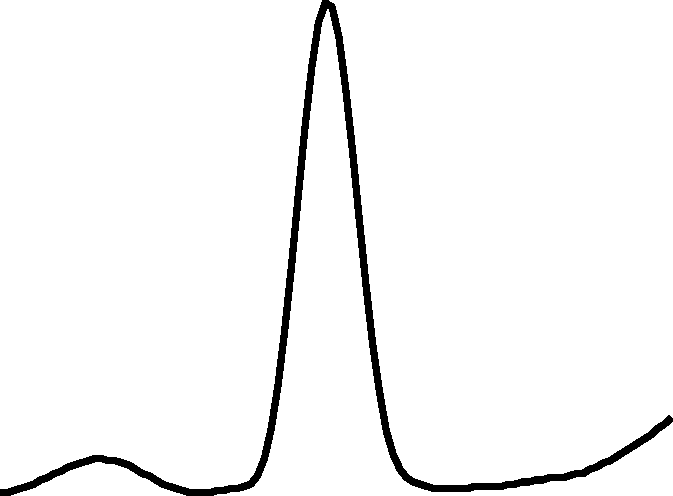
\includegraphics[scale=0.15]{figures/lowpass.pdf}
        \column{0.1\textwidth}
        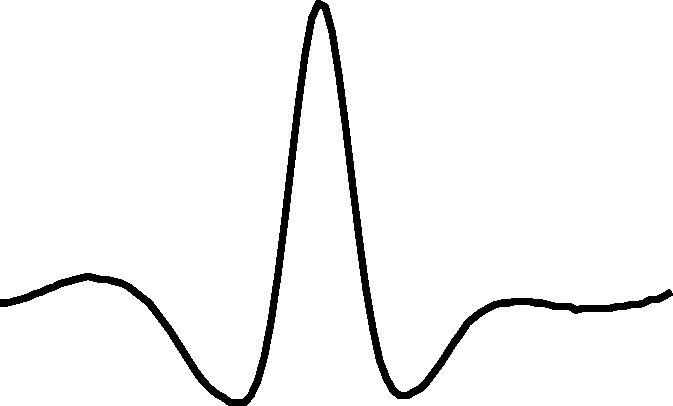
\includegraphics[scale=0.15]{figures/highpass.pdf}
        \column{0.1\textwidth}
        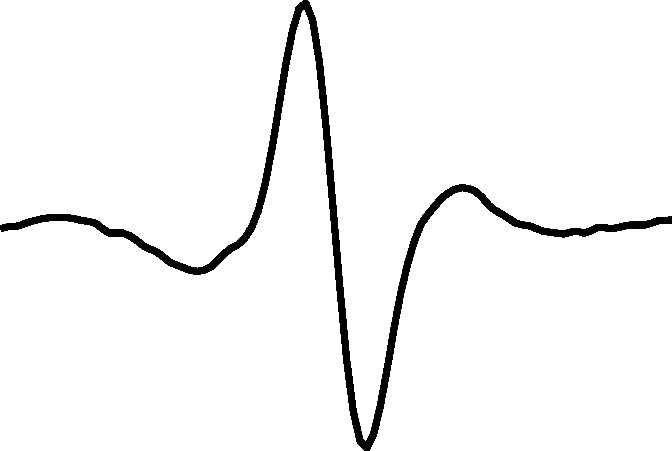
\includegraphics[scale=0.15]{figures/differentiator.pdf}
        \column{0.1\textwidth}
        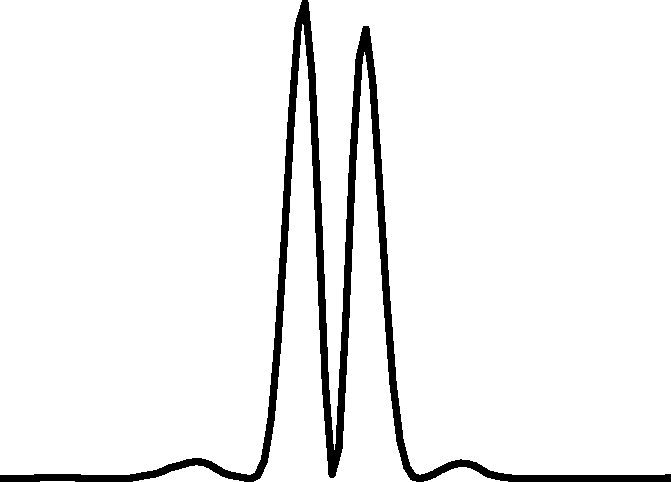
\includegraphics[scale=0.15]{figures/squaring.pdf}
        \column{0.1\textwidth}
        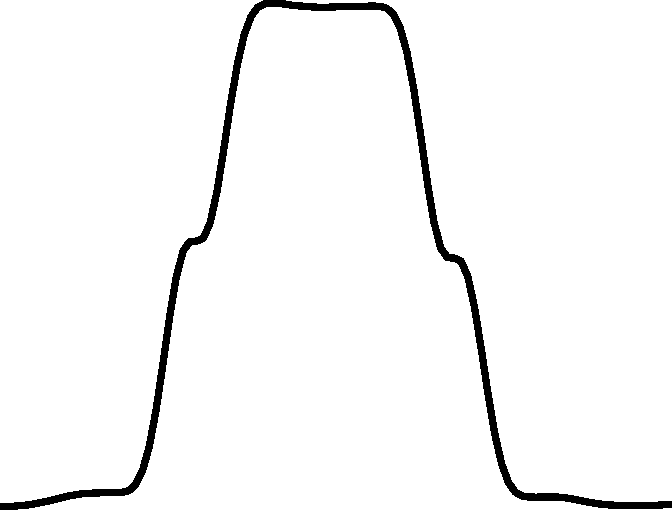
\includegraphics[scale=0.15]{figures/moving-average.pdf}
    \end{columns}
\end{frame}

\begin{frame}{Pré-processamento -- Detecção FP}
    \center
    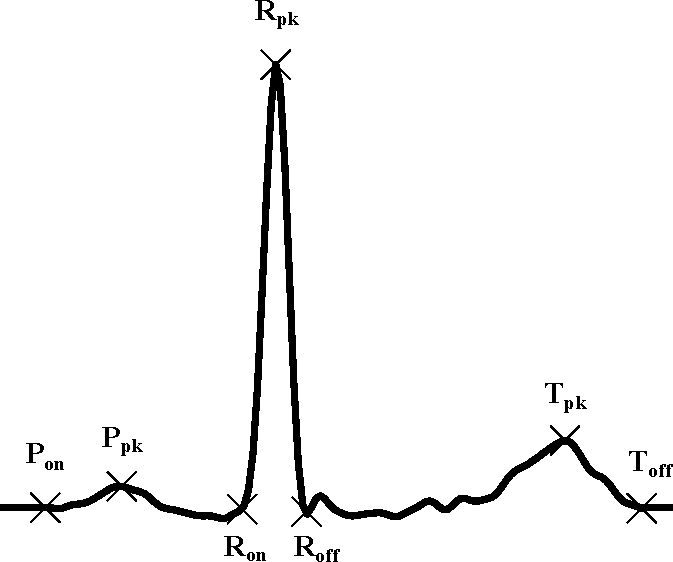
\includegraphics[scale=0.7]{figures/fiducial-points.pdf}
\end{frame}

\begin{frame}{Pré-processamento -- Linha de base}
    \begin{columns}
        \column{0.5\textwidth}
        \begin{tikzpicture}
            \node[anchor=south west,inner sep=0] at (0,0) {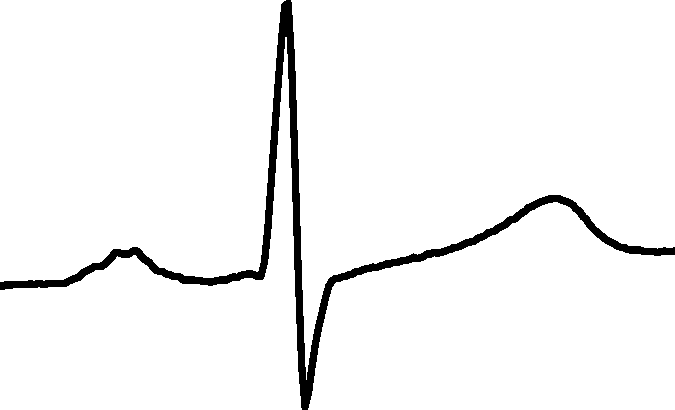
\includegraphics[width=\textwidth]{figures/baseline.pdf}};
            \draw<2->[red,thick] (0.0,1.1) -- (6.0,1.4);
            \draw<3>[red,thick,->] (4.5,1.0) arc (-180:-90:1.5);
        \end{tikzpicture}
        \vskip30pt\null
        \column{0.5\textwidth}
        \null\vskip30pt
        \visible<3>{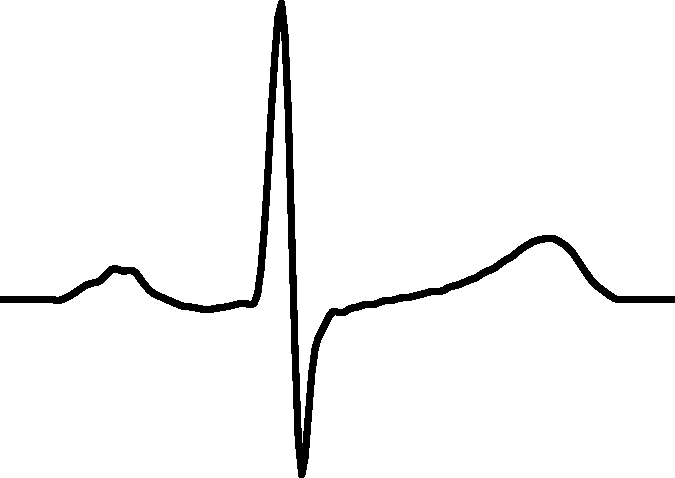
\includegraphics[scale=0.5]{figures/no-baseline.pdf}}
    \end{columns}
\end{frame}

\begin{frame}{Pré-processamento -- \emph{Template}}
    \begin{columns}
        \column{0.25\textwidth}
        \fbox{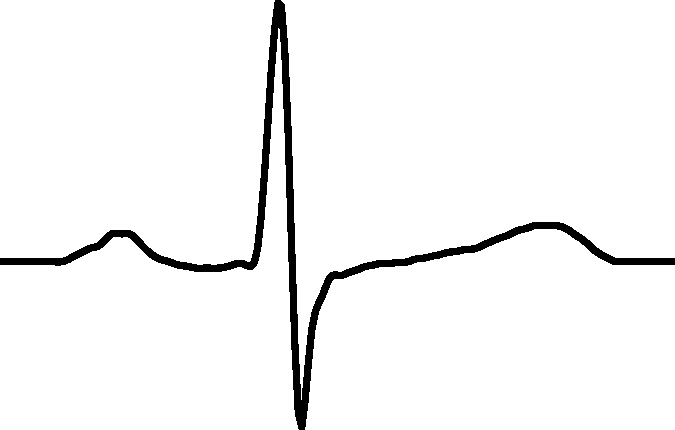
\includegraphics[scale=0.25]{figures/beat-sample.pdf}}
        \column{0.01\textwidth}
        $+$
        \column{0.25\textwidth}
        \fbox{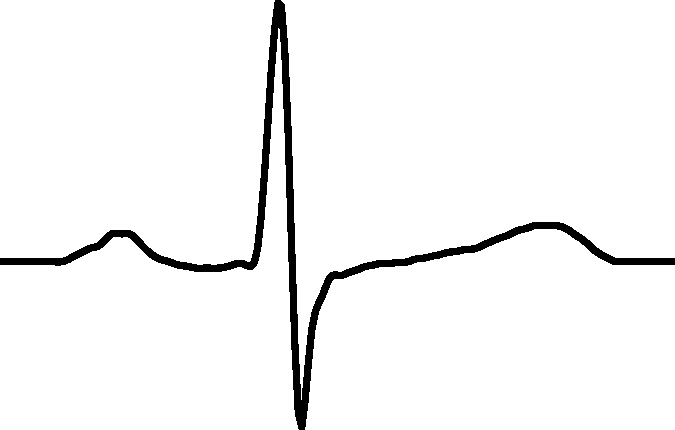
\includegraphics[scale=0.25]{figures/beat-sample.pdf}}
        \column{0.1\textwidth}
        $+\cdots+$
        \column{0.25\textwidth}
        \fbox{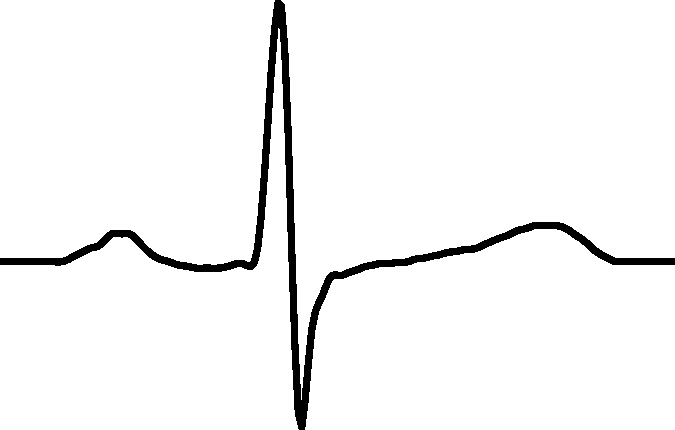
\includegraphics[scale=0.25]{figures/beat-sample.pdf}}
    \end{columns}
    \rule{\textwidth}{1pt}
    \centering{$N$}
    \vskip20pt
    \begin{columns}
        \column{0.1\textwidth}
        \column{0.01\textwidth}
        \visible<2>{$=$}
        \column{0.6\textwidth}
        \visible<2>{\fbox{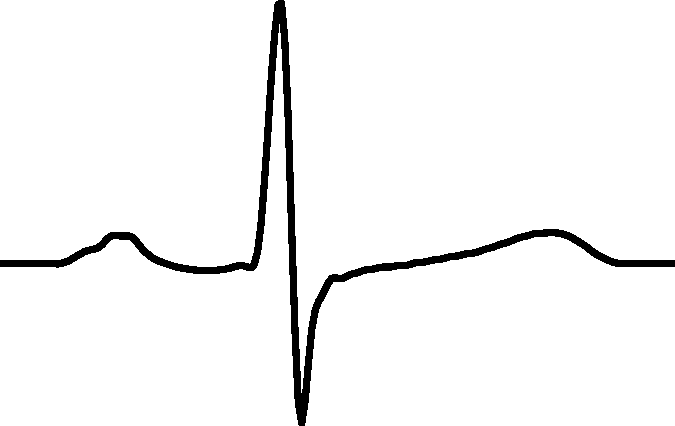
\includegraphics[scale=0.5]{figures/template.pdf}}}
    \end{columns}
\end{frame}

\begin{frame}{Pré-processamento -- Artefatos}
    \begin{columns}
        \column{0.4\textwidth}
        \fbox{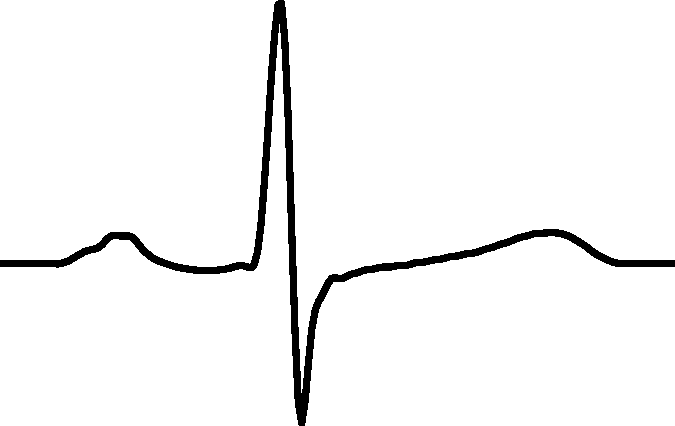
\includegraphics[scale=0.4]{figures/template.pdf}}
        \vskip10pt
        \fbox{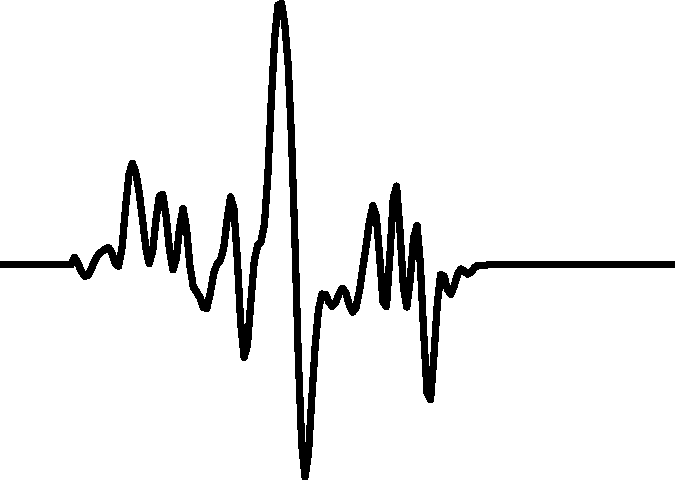
\includegraphics[scale=0.4]{figures/artifact.pdf}}
        \column{0.5\textwidth}
        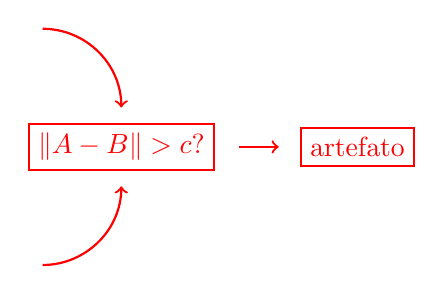
\begin{tikzpicture}
            \draw<2->[red,thick,->] (0.0,3.5) arc (90:0:1.0);
            \draw<2->[red,thick,->] (0.0,0.5) arc (-90:0:1.0);
            \node<2->[red,thick,draw,rectangle] at (1.0,2.0) {$\|A-B\|>c$?};
            \draw<3>[red,thick,->] (2.5,2.0) -- (3.0,2.0);
            \node<3>[red,thick,draw,rectangle] at (4.0,2.0) {artefato};
        \end{tikzpicture}
    \end{columns}
\end{frame}
